\documentclass[twoside]{book}

% Packages required by doxygen
\usepackage{fixltx2e}
\usepackage{calc}
\usepackage{doxygen}
\usepackage[export]{adjustbox} % also loads graphicx
\usepackage{graphicx}
\usepackage[utf8]{inputenc}
\usepackage{makeidx}
\usepackage{multicol}
\usepackage{multirow}
\PassOptionsToPackage{warn}{textcomp}
\usepackage{textcomp}
\usepackage[nointegrals]{wasysym}
\usepackage[table]{xcolor}

% Font selection
\usepackage[T1]{fontenc}
\usepackage[scaled=.90]{helvet}
\usepackage{courier}
\usepackage{amssymb}
\usepackage{sectsty}
\renewcommand{\familydefault}{\sfdefault}
\allsectionsfont{%
  \fontseries{bc}\selectfont%
  \color{darkgray}%
}
\renewcommand{\DoxyLabelFont}{%
  \fontseries{bc}\selectfont%
  \color{darkgray}%
}
\newcommand{\+}{\discretionary{\mbox{\scriptsize$\hookleftarrow$}}{}{}}

% Page & text layout
\usepackage{geometry}
\geometry{%
  a4paper,%
  top=2.5cm,%
  bottom=2.5cm,%
  left=2.5cm,%
  right=2.5cm%
}
\tolerance=750
\hfuzz=15pt
\hbadness=750
\setlength{\emergencystretch}{15pt}
\setlength{\parindent}{0cm}
\setlength{\parskip}{3ex plus 2ex minus 2ex}
\makeatletter
\renewcommand{\paragraph}{%
  \@startsection{paragraph}{4}{0ex}{-1.0ex}{1.0ex}{%
    \normalfont\normalsize\bfseries\SS@parafont%
  }%
}
\renewcommand{\subparagraph}{%
  \@startsection{subparagraph}{5}{0ex}{-1.0ex}{1.0ex}{%
    \normalfont\normalsize\bfseries\SS@subparafont%
  }%
}
\makeatother

% Headers & footers
\usepackage{fancyhdr}
\pagestyle{fancyplain}
\fancyhead[LE]{\fancyplain{}{\bfseries\thepage}}
\fancyhead[CE]{\fancyplain{}{}}
\fancyhead[RE]{\fancyplain{}{\bfseries\leftmark}}
\fancyhead[LO]{\fancyplain{}{\bfseries\rightmark}}
\fancyhead[CO]{\fancyplain{}{}}
\fancyhead[RO]{\fancyplain{}{\bfseries\thepage}}
\fancyfoot[LE]{\fancyplain{}{}}
\fancyfoot[CE]{\fancyplain{}{}}
\fancyfoot[RE]{\fancyplain{}{\bfseries\scriptsize Generated by Doxygen }}
\fancyfoot[LO]{\fancyplain{}{\bfseries\scriptsize Generated by Doxygen }}
\fancyfoot[CO]{\fancyplain{}{}}
\fancyfoot[RO]{\fancyplain{}{}}
\renewcommand{\footrulewidth}{0.4pt}
\renewcommand{\chaptermark}[1]{%
  \markboth{#1}{}%
}
\renewcommand{\sectionmark}[1]{%
  \markright{\thesection\ #1}%
}

% Indices & bibliography
\usepackage{natbib}
\usepackage[titles]{tocloft}
\setcounter{tocdepth}{3}
\setcounter{secnumdepth}{5}
\makeindex

% Hyperlinks (required, but should be loaded last)
\usepackage{ifpdf}
\ifpdf
  \usepackage[pdftex,pagebackref=true]{hyperref}
\else
  \usepackage[ps2pdf,pagebackref=true]{hyperref}
\fi
\hypersetup{%
  colorlinks=true,%
  linkcolor=blue,%
  citecolor=blue,%
  unicode%
}

% Custom commands
\newcommand{\clearemptydoublepage}{%
  \newpage{\pagestyle{empty}\cleardoublepage}%
}

\usepackage{caption}
\captionsetup{labelsep=space,justification=centering,font={bf},singlelinecheck=off,skip=4pt,position=top}

%===== C O N T E N T S =====

\begin{document}

% Titlepage & ToC
\hypersetup{pageanchor=false,
             bookmarksnumbered=true,
             pdfencoding=unicode
            }
\pagenumbering{roman}
\begin{titlepage}
\vspace*{7cm}
\begin{center}%
{\Large R\+T2-\/assignment-\/1 project \\[1ex]\large 0.\+0.\+1 }\\
\vspace*{1cm}
{\large Generated by Doxygen 1.8.11}\\
\end{center}
\end{titlepage}
\clearemptydoublepage
\tableofcontents
\clearemptydoublepage
\pagenumbering{arabic}
\hypersetup{pageanchor=true}

%--- Begin generated contents ---
\chapter{R\+E\+A\+D\+ME}
\label{md__root_Desktop_newassignment_rt2_assignment1_README}
\hypertarget{md__root_Desktop_newassignment_rt2_assignment1_README}{}
\input{md__root_Desktop_newassignment_rt2_assignment1_README}
\chapter{Namespace Index}
\doxysection{Namespace List}
Here is a list of all namespaces with brief descriptions\+:\begin{DoxyCompactList}
\item\contentsline{section}{\mbox{\hyperlink{namespaceconf}{conf}} }{\pageref{namespaceconf}}{}
\item\contentsline{section}{\mbox{\hyperlink{namespacego__to__point}{go\+\_\+to\+\_\+point}} }{\pageref{namespacego__to__point}}{}
\item\contentsline{section}{\mbox{\hyperlink{namespacert2__assignment1}{rt2\+\_\+assignment1}} }{\pageref{namespacert2__assignment1}}{}
\item\contentsline{section}{\mbox{\hyperlink{namespaceuser__interface}{user\+\_\+interface}} }{\pageref{namespaceuser__interface}}{}
\end{DoxyCompactList}

\chapter{Hierarchical Index}
\section{Class Hierarchy}
This inheritance list is sorted roughly, but not completely, alphabetically\+:\begin{DoxyCompactList}
\item object\begin{DoxyCompactList}
\item \contentsline{section}{go\+\_\+to\+\_\+point.\+Goal\+Reaching\+Action}{\pageref{classgo__to__point_1_1_goal_reaching_action}}{}
\end{DoxyCompactList}
\end{DoxyCompactList}

\chapter{Class Index}
\doxysection{Class List}
Here are the classes, structs, unions and interfaces with brief descriptions\+:\begin{DoxyCompactList}
\item\contentsline{section}{\mbox{\hyperlink{classgo__to__point_1_1_goal_reaching_action}{go\+\_\+to\+\_\+point.\+Goal\+Reaching\+Action}} }{\pageref{classgo__to__point_1_1_goal_reaching_action}}{}
\end{DoxyCompactList}

\chapter{File Index}
\section{File List}
Here is a list of all files with brief descriptions\+:\begin{DoxyCompactList}
\item\contentsline{section}{/root/\+Desktop/newassignment/rt2\+\_\+assignment1/launch/\hyperlink{all__launch_8py}{all\+\_\+launch.\+py} }{\pageref{all__launch_8py}}{}
\item\contentsline{section}{/root/\+Desktop/newassignment/rt2\+\_\+assignment1/src/\hyperlink{position__service_8cpp}{position\+\_\+service.\+cpp} }{\pageref{position__service_8cpp}}{}
\item\contentsline{section}{/root/\+Desktop/newassignment/rt2\+\_\+assignment1/src/\hyperlink{state__machine_8cpp}{state\+\_\+machine.\+cpp} }{\pageref{state__machine_8cpp}}{}
\end{DoxyCompactList}

\chapter{Namespace Documentation}
\hypertarget{namespaceall__launch}{}\section{all\+\_\+launch Namespace Reference}
\label{namespaceall__launch}\index{all\+\_\+launch@{all\+\_\+launch}}
\subsection*{Functions}
\begin{DoxyCompactItemize}
\item 
def \hyperlink{namespaceall__launch_adf61a15fe547d4d092b1cbd6a14ecff1}{generate\+\_\+launch\+\_\+description} ()
\end{DoxyCompactItemize}


\subsection{Function Documentation}
\index{all\+\_\+launch@{all\+\_\+launch}!generate\+\_\+launch\+\_\+description@{generate\+\_\+launch\+\_\+description}}
\index{generate\+\_\+launch\+\_\+description@{generate\+\_\+launch\+\_\+description}!all\+\_\+launch@{all\+\_\+launch}}
\subsubsection[{\texorpdfstring{generate\+\_\+launch\+\_\+description()}{generate_launch_description()}}]{\setlength{\rightskip}{0pt plus 5cm}def all\+\_\+launch.\+generate\+\_\+launch\+\_\+description (
\begin{DoxyParamCaption}
{}
\end{DoxyParamCaption}
)}\hypertarget{namespaceall__launch_adf61a15fe547d4d092b1cbd6a14ecff1}{}\label{namespaceall__launch_adf61a15fe547d4d092b1cbd6a14ecff1}
\begin{DoxyVerb}Generate launch description with multiple components.\end{DoxyVerb}
 

Definition at line 5 of file all\+\_\+launch.\+py.


\hypertarget{namespacert2__assignment1}{}\section{rt2\+\_\+assignment1 Namespace Reference}
\label{namespacert2__assignment1}\index{rt2\+\_\+assignment1@{rt2\+\_\+assignment1}}
\subsection*{Classes}
\begin{DoxyCompactItemize}
\item 
class \hyperlink{classrt2__assignment1_1_1_f_s_m}{F\+SM}
\item 
class \hyperlink{classrt2__assignment1_1_1_position___service}{Position\+\_\+\+Service}
\end{DoxyCompactItemize}

\chapter{Class Documentation}
\hypertarget{classrt2__assignment1_1_1_f_s_m}{}\section{rt2\+\_\+assignment1\+:\+:F\+SM Class Reference}
\label{classrt2__assignment1_1_1_f_s_m}\index{rt2\+\_\+assignment1\+::\+F\+SM@{rt2\+\_\+assignment1\+::\+F\+SM}}


Inheritance diagram for rt2\+\_\+assignment1\+:\+:F\+SM\+:
\nopagebreak
\begin{figure}[H]
\begin{center}
\leavevmode
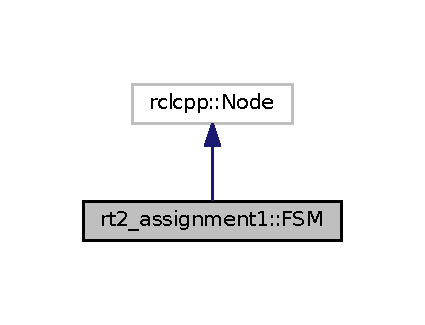
\includegraphics[width=204pt]{classrt2__assignment1_1_1_f_s_m__inherit__graph}
\end{center}
\end{figure}


Collaboration diagram for rt2\+\_\+assignment1\+:\+:F\+SM\+:
\nopagebreak
\begin{figure}[H]
\begin{center}
\leavevmode
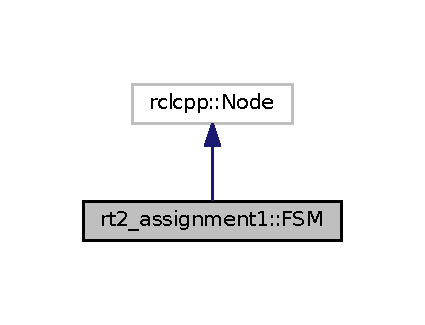
\includegraphics[width=204pt]{classrt2__assignment1_1_1_f_s_m__coll__graph}
\end{center}
\end{figure}
\subsection*{Public Member Functions}
\begin{DoxyCompactItemize}
\item 
\hyperlink{classrt2__assignment1_1_1_f_s_m_a478e9cd5058c96962f690993f8c28517}{F\+SM} (const rclcpp\+::\+Node\+Options \&options)
\end{DoxyCompactItemize}


\subsection{Detailed Description}
\hyperlink{classrt2__assignment1_1_1_f_s_m}{F\+SM} (Finite State Machine) Class\+: The \hyperlink{classrt2__assignment1_1_1_f_s_m}{F\+SM} Node is implemented as a class so that it can be structured as a component. Indeed, it shall communicates with the ros node by means of the ros1\+\_\+bridge package 

Definition at line 26 of file state\+\_\+machine.\+cpp.



\subsection{Constructor \& Destructor Documentation}
\index{rt2\+\_\+assignment1\+::\+F\+SM@{rt2\+\_\+assignment1\+::\+F\+SM}!F\+SM@{F\+SM}}
\index{F\+SM@{F\+SM}!rt2\+\_\+assignment1\+::\+F\+SM@{rt2\+\_\+assignment1\+::\+F\+SM}}
\subsubsection[{\texorpdfstring{F\+S\+M(const rclcpp\+::\+Node\+Options \&options)}{FSM(const rclcpp::NodeOptions &options)}}]{\setlength{\rightskip}{0pt plus 5cm}rt2\+\_\+assignment1\+::\+F\+S\+M\+::\+F\+SM (
\begin{DoxyParamCaption}
\item[{const rclcpp\+::\+Node\+Options \&}]{options}
\end{DoxyParamCaption}
)\hspace{0.3cm}{\ttfamily [inline]}}\hypertarget{classrt2__assignment1_1_1_f_s_m_a478e9cd5058c96962f690993f8c28517}{}\label{classrt2__assignment1_1_1_f_s_m_a478e9cd5058c96962f690993f8c28517}
Initialisation of the state\+\_\+machine service and clients. Inside the Class constructor, there exists a /user\+\_\+interface service. By means of the bind function, the callback is executed as soon as the client makes a request. Then the \hyperlink{classrt2__assignment1_1_1_f_s_m}{F\+SM} starts working. $<$ server of type Command

$<$ client\+\_\+1 of type position

$<$ client\+\_\+2 of type Random\+Position 

Definition at line 34 of file state\+\_\+machine.\+cpp.



The documentation for this class was generated from the following file\+:\begin{DoxyCompactItemize}
\item 
/root/\+Desktop/newassignment/rt2\+\_\+assignment1/src/\hyperlink{state__machine_8cpp}{state\+\_\+machine.\+cpp}\end{DoxyCompactItemize}

\hypertarget{classrt2__assignment1_1_1_position___service}{}\section{rt2\+\_\+assignment1\+:\+:Position\+\_\+\+Service Class Reference}
\label{classrt2__assignment1_1_1_position___service}\index{rt2\+\_\+assignment1\+::\+Position\+\_\+\+Service@{rt2\+\_\+assignment1\+::\+Position\+\_\+\+Service}}


Inheritance diagram for rt2\+\_\+assignment1\+:\+:Position\+\_\+\+Service\+:
\nopagebreak
\begin{figure}[H]
\begin{center}
\leavevmode
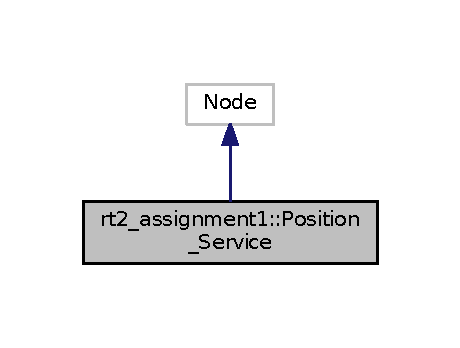
\includegraphics[width=221pt]{classrt2__assignment1_1_1_position___service__inherit__graph}
\end{center}
\end{figure}


Collaboration diagram for rt2\+\_\+assignment1\+:\+:Position\+\_\+\+Service\+:
\nopagebreak
\begin{figure}[H]
\begin{center}
\leavevmode
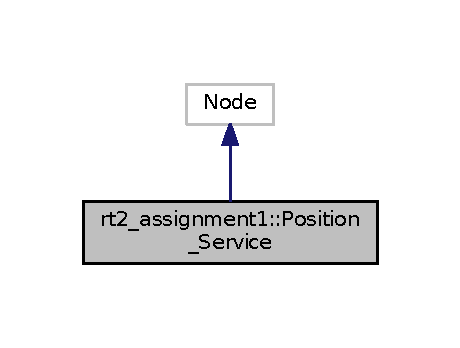
\includegraphics[width=221pt]{classrt2__assignment1_1_1_position___service__coll__graph}
\end{center}
\end{figure}
\subsection*{Public Member Functions}
\begin{DoxyCompactItemize}
\item 
\hyperlink{classrt2__assignment1_1_1_position___service_ae2e368da61b80e1cae13836801ec907c}{Position\+\_\+\+Service} (const rclcpp\+::\+Node\+Options \&options)
\end{DoxyCompactItemize}


\subsection{Detailed Description}
Position\+\_\+service Class\+: The position\+\_\+service Node is implemented as a class so that it can be structured as a component. Indeed, it shall communicates with the ros node by means of the ros1\+\_\+bridge package 

Definition at line 20 of file position\+\_\+service.\+cpp.



\subsection{Constructor \& Destructor Documentation}
\index{rt2\+\_\+assignment1\+::\+Position\+\_\+\+Service@{rt2\+\_\+assignment1\+::\+Position\+\_\+\+Service}!Position\+\_\+\+Service@{Position\+\_\+\+Service}}
\index{Position\+\_\+\+Service@{Position\+\_\+\+Service}!rt2\+\_\+assignment1\+::\+Position\+\_\+\+Service@{rt2\+\_\+assignment1\+::\+Position\+\_\+\+Service}}
\subsubsection[{\texorpdfstring{Position\+\_\+\+Service(const rclcpp\+::\+Node\+Options \&options)}{Position_Service(const rclcpp::NodeOptions &options)}}]{\setlength{\rightskip}{0pt plus 5cm}rt2\+\_\+assignment1\+::\+Position\+\_\+\+Service\+::\+Position\+\_\+\+Service (
\begin{DoxyParamCaption}
\item[{const rclcpp\+::\+Node\+Options \&}]{options}
\end{DoxyParamCaption}
)\hspace{0.3cm}{\ttfamily [inline]}}\hypertarget{classrt2__assignment1_1_1_position___service_ae2e368da61b80e1cae13836801ec907c}{}\label{classrt2__assignment1_1_1_position___service_ae2e368da61b80e1cae13836801ec907c}
Initialisation of the random Position service. It takes as argument the callback and the three message fields by means of the bind function, the callback is executed as soon as the client makes a request. $<$ callback 

Definition at line 28 of file position\+\_\+service.\+cpp.



The documentation for this class was generated from the following file\+:\begin{DoxyCompactItemize}
\item 
/root/\+Desktop/newassignment/rt2\+\_\+assignment1/src/\hyperlink{position__service_8cpp}{position\+\_\+service.\+cpp}\end{DoxyCompactItemize}

\chapter{File Documentation}
\hypertarget{all__launch_8py}{}\section{/root/\+Desktop/newassignment/rt2\+\_\+assignment1/launch/all\+\_\+launch.py File Reference}
\label{all__launch_8py}\index{/root/\+Desktop/newassignment/rt2\+\_\+assignment1/launch/all\+\_\+launch.\+py@{/root/\+Desktop/newassignment/rt2\+\_\+assignment1/launch/all\+\_\+launch.\+py}}
\subsection*{Namespaces}
\begin{DoxyCompactItemize}
\item 
 \hyperlink{namespaceall__launch}{all\+\_\+launch}
\end{DoxyCompactItemize}
\subsection*{Functions}
\begin{DoxyCompactItemize}
\item 
def \hyperlink{namespaceall__launch_adf61a15fe547d4d092b1cbd6a14ecff1}{all\+\_\+launch.\+generate\+\_\+launch\+\_\+description} ()
\end{DoxyCompactItemize}

\hypertarget{_r_e_a_d_m_e_8md}{}\doxysection{R\+E\+A\+D\+M\+E.\+md File Reference}
\label{_r_e_a_d_m_e_8md}\index{README.md@{README.md}}

\hypertarget{position__service_8cpp}{}\doxysection{src/position\+\_\+service.cpp File Reference}
\label{position__service_8cpp}\index{src/position\_service.cpp@{src/position\_service.cpp}}


Node implementing the R\+OS service for getting random position.  


{\ttfamily \#include \char`\"{}ros/ros.\+h\char`\"{}}\newline
{\ttfamily \#include \char`\"{}rt2\+\_\+assignment1/\+Random\+Position.\+h\char`\"{}}\newline
Include dependency graph for position\+\_\+service.\+cpp\+:
\nopagebreak
\begin{figure}[H]
\begin{center}
\leavevmode
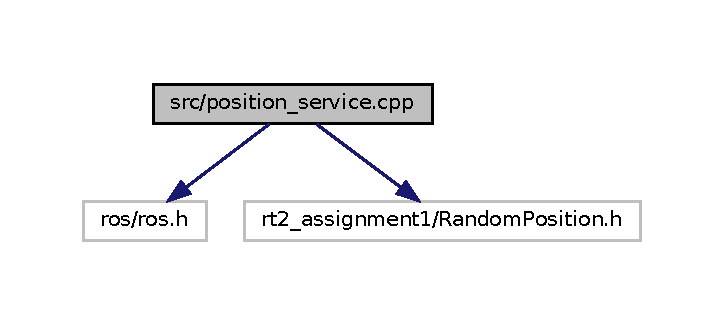
\includegraphics[width=348pt]{position__service_8cpp__incl}
\end{center}
\end{figure}
\doxysubsection*{Namespaces}
\begin{DoxyCompactItemize}
\item 
 \mbox{\hyperlink{namespacert2__assignment1}{rt2\+\_\+assignment1}}
\end{DoxyCompactItemize}
\doxysubsection*{Functions}
\begin{DoxyCompactItemize}
\item 
double \mbox{\hyperlink{position__service_8cpp_a10f83119b77a8fbd085a5550955f85ff}{rand\+M\+ToN}} (double M, double N)
\begin{DoxyCompactList}\small\item\em Random number generator. \end{DoxyCompactList}\item 
bool \mbox{\hyperlink{position__service_8cpp_ab65b9ff5368189ad34fe4989d50742e4}{myrandom}} (rt2\+\_\+assignment1\+::\+Random\+Position\+::\+Request \&req, rt2\+\_\+assignment1\+::\+Random\+Position\+::\+Response \&res)
\begin{DoxyCompactList}\small\item\em This function is the callback of the service server. \end{DoxyCompactList}\item 
int \mbox{\hyperlink{position__service_8cpp_a3c04138a5bfe5d72780bb7e82a18e627}{main}} (int argc, char $\ast$$\ast$argv)
\begin{DoxyCompactList}\small\item\em main function \end{DoxyCompactList}\end{DoxyCompactItemize}


\doxysubsection{Detailed Description}
Node implementing the R\+OS service for getting random position. 

\begin{DoxyAuthor}{Author}
Federico Civetta 
\end{DoxyAuthor}
\begin{DoxyVersion}{Version}
0.\+1 
\end{DoxyVersion}
\begin{DoxyDate}{Date}
13/06/2021
\end{DoxyDate}
Subscribes to\+: ~\newline
 None

Publishes to\+: ~\newline
 None

Services\+: ~\newline
 /position\+\_\+server

Description\+: ~\newline


This node advertises a position service. When the service is require, a request containing the minimum and the maximum values for the x and y position is used to generate a random position between x (or y) min and x (or y) max. 

\doxysubsection{Function Documentation}
\mbox{\Hypertarget{position__service_8cpp_a3c04138a5bfe5d72780bb7e82a18e627}\label{position__service_8cpp_a3c04138a5bfe5d72780bb7e82a18e627}} 
\index{position\_service.cpp@{position\_service.cpp}!main@{main}}
\index{main@{main}!position\_service.cpp@{position\_service.cpp}}
\doxysubsubsection{\texorpdfstring{main()}{main()}}
{\footnotesize\ttfamily int main (\begin{DoxyParamCaption}\item[{int}]{argc,  }\item[{char $\ast$$\ast$}]{argv }\end{DoxyParamCaption})}



main function 


\begin{DoxyRetVals}{Return values}
{\em 0} & This function initializes the server /position\+\_\+server, and the ros node (random\+\_\+position\+\_\+server) Then, while running, it waits for a request adressed to the server \\
\hline
\end{DoxyRetVals}


Definition at line 76 of file position\+\_\+service.\+cpp.

\mbox{\Hypertarget{position__service_8cpp_ab65b9ff5368189ad34fe4989d50742e4}\label{position__service_8cpp_ab65b9ff5368189ad34fe4989d50742e4}} 
\index{position\_service.cpp@{position\_service.cpp}!myrandom@{myrandom}}
\index{myrandom@{myrandom}!position\_service.cpp@{position\_service.cpp}}
\doxysubsubsection{\texorpdfstring{myrandom()}{myrandom()}}
{\footnotesize\ttfamily bool myrandom (\begin{DoxyParamCaption}\item[{rt2\+\_\+assignment1\+::\+Random\+Position\+::\+Request \&}]{req,  }\item[{rt2\+\_\+assignment1\+::\+Random\+Position\+::\+Response \&}]{res }\end{DoxyParamCaption})}



This function is the callback of the service server. 


\begin{DoxyParams}{Parameters}
{\em req} & the request received from the client. It gets two intervals of values for x and y \\
\hline
{\em res} & the response returned to the client (the random coordinates within a specific interval)\\
\hline
\end{DoxyParams}

\begin{DoxyRetVals}{Return values}
{\em the} & boolean True\\
\hline
\end{DoxyRetVals}
This function exploits the rand function, which returns a pseudo-\/random integral number in the range between 0 and R\+A\+N\+D\+\_\+\+M\+AX. It is called when a request from the client is received. 

Definition at line 58 of file position\+\_\+service.\+cpp.

\mbox{\Hypertarget{position__service_8cpp_a10f83119b77a8fbd085a5550955f85ff}\label{position__service_8cpp_a10f83119b77a8fbd085a5550955f85ff}} 
\index{position\_service.cpp@{position\_service.cpp}!randMToN@{randMToN}}
\index{randMToN@{randMToN}!position\_service.cpp@{position\_service.cpp}}
\doxysubsubsection{\texorpdfstring{randMToN()}{randMToN()}}
{\footnotesize\ttfamily double rand\+M\+ToN (\begin{DoxyParamCaption}\item[{double}]{M,  }\item[{double}]{N }\end{DoxyParamCaption})}



Random number generator. 


\begin{DoxyParams}{Parameters}
{\em M} & defines the minimum possible value for a random number (within a certain interval) \\
\hline
{\em N} & the maximum possible value for a random number (within a certain interval)\\
\hline
\end{DoxyParams}

\begin{DoxyRetVals}{Return values}
{\em a} & double value, defining a random number adressed to myrandom\\
\hline
\end{DoxyRetVals}
This function generates a random number between M and N 

Definition at line 44 of file position\+\_\+service.\+cpp.


\hypertarget{state__machine_8cpp}{}\section{src/state\+\_\+machine.cpp File Reference}
\label{state__machine_8cpp}\index{src/state\+\_\+machine.\+cpp@{src/state\+\_\+machine.\+cpp}}
{\ttfamily \#include \char`\"{}ros/ros.\+h\char`\"{}}\\*
{\ttfamily \#include \char`\"{}rt2\+\_\+assignment1/\+Command.\+h\char`\"{}}\\*
{\ttfamily \#include \char`\"{}rt2\+\_\+assignment1/\+Random\+Position.\+h\char`\"{}}\\*
{\ttfamily \#include $<$actionlib/client/simple\+\_\+action\+\_\+client.\+h$>$}\\*
{\ttfamily \#include $<$actionlib/client/terminal\+\_\+state.\+h$>$}\\*
{\ttfamily \#include $<$rt2\+\_\+assignment1/\+Goal\+Reaching\+Action.\+h$>$}\\*
Include dependency graph for state\+\_\+machine.\+cpp\+:\nopagebreak
\begin{figure}[H]
\begin{center}
\leavevmode
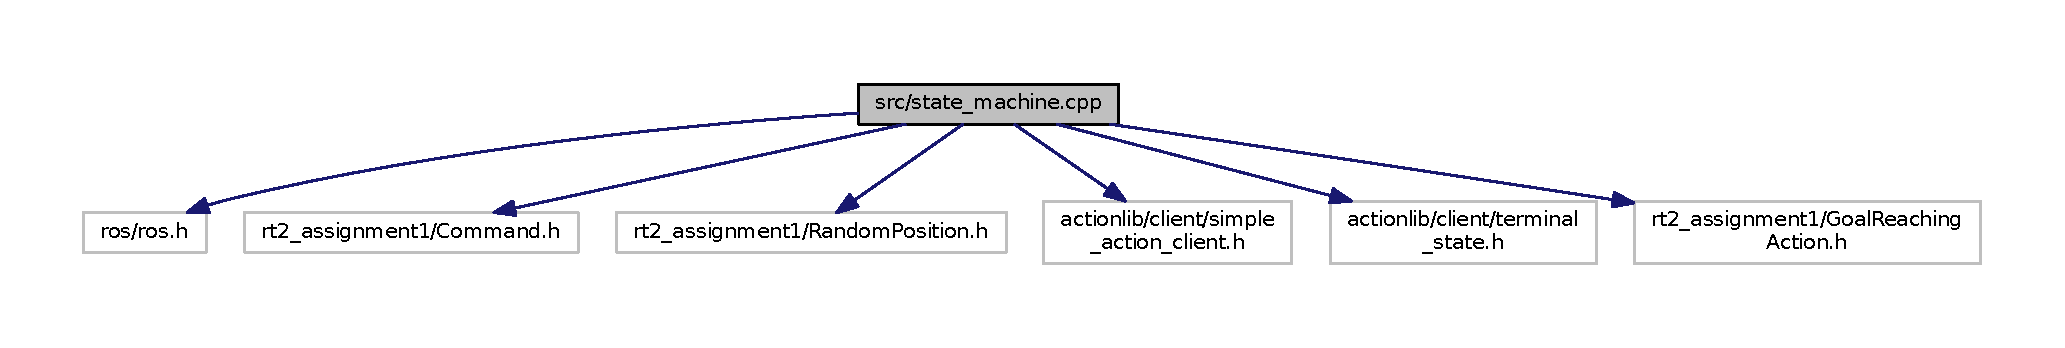
\includegraphics[width=350pt]{state__machine_8cpp__incl}
\end{center}
\end{figure}
\subsection*{Functions}
\begin{DoxyCompactItemize}
\item 
bool \hyperlink{state__machine_8cpp_a1a9543636935547580c0657f4c7c0c2b}{user\+\_\+interface} (rt2\+\_\+assignment1\+::\+Command\+::\+Request \&req, rt2\+\_\+assignment1\+::\+Command\+::\+Response \&res)
\begin{DoxyCompactList}\small\item\em This function is the callback function of the servise for server. \end{DoxyCompactList}\item 
int \hyperlink{state__machine_8cpp_a3c04138a5bfe5d72780bb7e82a18e627}{main} (int argc, char $\ast$$\ast$argv)
\end{DoxyCompactItemize}
\subsection*{Variables}
\begin{DoxyCompactItemize}
\item 
bool \hyperlink{state__machine_8cpp_ab376b87f96a574a793c03c53e75afec8}{start} = false
\end{DoxyCompactItemize}


\subsection{Function Documentation}
\index{state\+\_\+machine.\+cpp@{state\+\_\+machine.\+cpp}!main@{main}}
\index{main@{main}!state\+\_\+machine.\+cpp@{state\+\_\+machine.\+cpp}}
\subsubsection[{\texorpdfstring{main(int argc, char $\ast$$\ast$argv)}{main(int argc, char **argv)}}]{\setlength{\rightskip}{0pt plus 5cm}int main (
\begin{DoxyParamCaption}
\item[{int}]{argc, }
\item[{char $\ast$$\ast$}]{argv}
\end{DoxyParamCaption}
)}\hypertarget{state__machine_8cpp_a3c04138a5bfe5d72780bb7e82a18e627}{}\label{state__machine_8cpp_a3c04138a5bfe5d72780bb7e82a18e627}


Definition at line 33 of file state\+\_\+machine.\+cpp.

\index{state\+\_\+machine.\+cpp@{state\+\_\+machine.\+cpp}!user\+\_\+interface@{user\+\_\+interface}}
\index{user\+\_\+interface@{user\+\_\+interface}!state\+\_\+machine.\+cpp@{state\+\_\+machine.\+cpp}}
\subsubsection[{\texorpdfstring{user\+\_\+interface(rt2\+\_\+assignment1\+::\+Command\+::\+Request \&req, rt2\+\_\+assignment1\+::\+Command\+::\+Response \&res)}{user_interface(rt2_assignment1::Command::Request &req, rt2_assignment1::Command::Response &res)}}]{\setlength{\rightskip}{0pt plus 5cm}bool user\+\_\+interface (
\begin{DoxyParamCaption}
\item[{rt2\+\_\+assignment1\+::\+Command\+::\+Request \&}]{req, }
\item[{rt2\+\_\+assignment1\+::\+Command\+::\+Response \&}]{res}
\end{DoxyParamCaption}
)}\hypertarget{state__machine_8cpp_a1a9543636935547580c0657f4c7c0c2b}{}\label{state__machine_8cpp_a1a9543636935547580c0657f4c7c0c2b}


This function is the callback function of the servise for server. 


\begin{DoxyParams}{Parameters}
{\em req} & the request received from the client of the \hyperlink{user__interface_8py}{user\+\_\+interface.\+py}. \\
\hline
{\em res} & the response has not been used \\
\hline
\end{DoxyParams}

\begin{DoxyRetVals}{Return values}
{\em A} & boolean value \\
\hline
\end{DoxyRetVals}


Definition at line 17 of file state\+\_\+machine.\+cpp.



\subsection{Variable Documentation}
\index{state\+\_\+machine.\+cpp@{state\+\_\+machine.\+cpp}!start@{start}}
\index{start@{start}!state\+\_\+machine.\+cpp@{state\+\_\+machine.\+cpp}}
\subsubsection[{\texorpdfstring{start}{start}}]{\setlength{\rightskip}{0pt plus 5cm}bool start = false}\hypertarget{state__machine_8cpp_ab376b87f96a574a793c03c53e75afec8}{}\label{state__machine_8cpp_ab376b87f96a574a793c03c53e75afec8}


Definition at line 8 of file state\+\_\+machine.\+cpp.


%--- End generated contents ---

% Index
\backmatter
\newpage
\phantomsection
\clearemptydoublepage
\addcontentsline{toc}{chapter}{Index}
\printindex

\end{document}
